\documentclass[10pt, a4paper]{report}
\usepackage[utf8]{inputenc}
\usepackage{booktabs}
\usepackage{multirow}
\usepackage[table,xcdraw]{xcolor}
\usepackage{adjustbox,lipsum}
\usepackage{csquotes}
\usepackage{graphicx}
\usepackage[linktoc=all]{hyperref}

\hypersetup{
    colorlinks,
    citecolor=black,
    filecolor=black,
    linkcolor=black,
    urlcolor=black
}

\newcommand{\myparagraph}[1]{\paragraph{#1}\mbox{}\\} %used for better formating of some text

\setlength{\oddsidemargin}{0cm}
\setlength{\evensidemargin}{0cm}
\setlength{\textwidth}{500pt}

\title{Review and comparison of tools for managing X.509 type keys and certificates}
\author{Oliver Bodnár}
\date{November 2016}

\begin{document}

\maketitle

\tableofcontents

\newpage

\part{Introduction}

Primary goal of this work is to compare and review some of the basic functionalities \textit{(e.g. generation of keys and certificates, ability to create a certificate signing request,...)} of tools working with keys and certificates in X.509 public key infrastructure. Comparison of tools is necessary to understand that ability of a tool to do everything that was tested does not mean that it is the best tool to use in every situation.
\part{Overview}

\chapter{Overview Tables}

\section{General}
\begin{table}[h!]
\centering
\caption{Overwiew General}
\label{my-label}
\begin{adjustbox}{max width=\textwidth}
\begin{tabular}{|c|c|c|c|c|c|}
\hline
                              & \multicolumn{5}{c|}{General}                                                                                   \\ \cline{2-6} 
\multirow{-2}{*}{Tools}       & Type   & View information about certificate                 & License & Operating System                        & Tool Type           \\ \hline
OpenSSL                       & PKCS12 & \cellcolor[HTML]{34FF34}Yes                        & Public  & \cellcolor[HTML]{34FF34}All             & Command Line        \\ \hline
Keytool                       & JKS    & \cellcolor[HTML]{34FF34}{\color[HTML]{000000} Yes} & Public  & \cellcolor[HTML]{34FF34}All             & Command Line        \\ \hline
GnuPG                         & None   & \cellcolor[HTML]{FE0000}No                         & Public  & \cellcolor[HTML]{34FF34}All             & Command Line        \\ \hline
Keystore Explorer             & Both   & \cellcolor[HTML]{34FF34}Yes                        & Public  & \cellcolor[HTML]{FFC702}Win $\vert$ OSX & Graphical Interface \\ \hline
XCA                           & PKCS12 & \cellcolor[HTML]{34FF34}Yes                        & Public  & \cellcolor[HTML]{34FF34}All             & Graphical Interface \\ \hline
GnuTLS                        & PKCS12 & \cellcolor[HTML]{34FF34}Yes                        & Public  & \cellcolor[HTML]{FFC702}UNIX            & Command Line        \\ \hline
Makecert and pvk2pfx          & PKCS12 & \cellcolor[HTML]{FE0000}No			    & Public  & \cellcolor[HTML]{FFC702}Windows         & Command Line        \\ \hline
Windows PowerShell PKI Module & PKCS12 & \cellcolor[HTML]{34FF34}Yes			    & Public  & \cellcolor[HTML]{FFC702}Windows         & Command Line        \\ \hline
\end{tabular}
\end{adjustbox}
\end{table}
%TABLE END

\subsection{Type}
This section defines type of storage file in which the certificates or keys are saved. 
Options are:
    \begin{itemize}
     \item \textit{PKCS\#12} - PKCS\#12 encoded file, usual extensions are \verb+.pfx+ and \verb+.p12+
     \item \textit{JKS} - Java KeyStore type file, usual extension is \verb+.jks+
    \end{itemize}

\subsection{View information about certificate}
This section shows whether it is possible to view information certificates and keys and additional information. 
    \begin{itemize}
     \item \textit{Yes} - viewing information about certificates and keys is availiable. This includes length, used algorithm, fingerprint.
     \item \textit{No}  - tool does not have an option to view any information about certificates or keys.
    \end{itemize}

\subsection{License}
Type of license and possibility of using said tool for testing or production code. 
    \begin{itemize}
     \item \textit{Public} - No restrictions for usage, can be used commercialy.
     \item \textit{Testing} - Tool is free to use non-commercialy. For commercial acquisition of paid license is needed.
     \item \textit{Paid} - Every type of usage is paid for. Restrictive version of product may be available, but to use all the features and be able to use in commercial enviroment paid license is needed.
    \end{itemize}

Public does not mean that it should be used as such. Definition if it is advised to use said tool in production code or only in testing enviroment will be talked about in next chapters under each tool.

\subsection{Operating Systems}
In this part the Operating System under which the tool is implemented is defined. 
    \begin{itemize}
     \item \textit{OS X $\vert$ Windows $\vert$ LINUX} - Tool is implemented under any of the mentioned OS, \verb+LINUX+ defines most common distributions of Linux systems \textit{(Debian or RPM based)}.
     \item \textit{UNIX} - Tool is implemented under UNIX-like systems, which is same as \textit{OS X $\vert$ LINUX} option.
     \item \textit{All} - Tool is implemented under every aforementioned operating system.
    \end{itemize}

\subsection{Tool Type}
This section shows what type of input is used in Tool. 
\begin{itemize}
\item \textit{Command Line} - tool is used with commands on some sort of console (PowerShell, Command Prompt, Terminal)
\item \textit{Graphical Interface} - tool is used with Graphical Interface, main interaction is by user using mouse
\end{itemize}
\newpage

\section{Generation and signing of certificates}

\subsection{Keys, certificates and basic constraints}
%TABLE START
\begin{table}[h!]
\centering
\caption{Generation of keys and certificates and basic constrints}
\begin{adjustbox}{max width=\textwidth}
\begin{tabular}{|c|c|c|c|c|c|c|}
\hline
                              & \multicolumn{4}{c|}{Generate keys}                                                                                                                             & \multicolumn{2}{c|}{Basic Constraints}                    \\ \cline{2-7} 
\multirow{-2}{*}{Tool}        & \begin{tabular}[c]{@{}c@{}}     self-signed certificate\end{tabular} &   CSR                       & Specify length              & Specify algorithm           & Specify Type                & Specify path length         \\ \hline
OpenSSL                       & \cellcolor[HTML]{34FF34}Yes                                          & \cellcolor[HTML]{34FF34}Yes & \cellcolor[HTML]{34FF34}Yes & \cellcolor[HTML]{34FF34}Yes & \cellcolor[HTML]{34FF34}Yes & \cellcolor[HTML]{34FF34}Yes \\ \hline
Keytool                       & \cellcolor[HTML]{34FF34}Yes                                          & \cellcolor[HTML]{34FF34}Yes & \cellcolor[HTML]{34FF34}Yes & \cellcolor[HTML]{34FF34}Yes & \cellcolor[HTML]{34FF34}Yes & \cellcolor[HTML]{34FF34}Yes \\ \hline
GnuPG                         & \cellcolor[HTML]{FE0000}No                                           & \cellcolor[HTML]{34FF34}Yes & \cellcolor[HTML]{FE0000} No & \cellcolor[HTML]{FE0000}No  & \cellcolor[HTML]{FE0000}No  & \cellcolor[HTML]{FE0000}No  \\ \hline
Keystore explorer             & \cellcolor[HTML]{34FF34}Yes                                          & \cellcolor[HTML]{34FF34}Yes & \cellcolor[HTML]{34FF34}Yes & \cellcolor[HTML]{34FF34}Yes & \cellcolor[HTML]{34FF34}Yes & \cellcolor[HTML]{34FF34}Yes \\ \hline
XCA                           & \cellcolor[HTML]{34FF34}Yes                                          & \cellcolor[HTML]{34FF34}Yes & \cellcolor[HTML]{34FF34}Yes & \cellcolor[HTML]{34FF34}Yes & \cellcolor[HTML]{34FF34}Yes & \cellcolor[HTML]{34FF34}Yes \\ \hline
GnuTLS                        & \cellcolor[HTML]{34FF34}Yes                                          & \cellcolor[HTML]{34FF34}Yes & \cellcolor[HTML]{34FF34}Yes & \cellcolor[HTML]{34FF34}Yes & \cellcolor[HTML]{34FF34}Yes & \cellcolor[HTML]{34FF34}Yes \\ \hline
Makecert and pvk2pfx          & \cellcolor[HTML]{34FF34}Yes					     & \cellcolor[HTML]{FE0000}No  & \cellcolor[HTML]{34FF34}Yes & \cellcolor[HTML]{FFC702}Yes & \cellcolor[HTML]{34FF34}Yes & \cellcolor[HTML]{34FF34}Yes \\ \hline
Windows PowerShell PKI Module & \cellcolor[HTML]{34FF34}Yes                                          & \cellcolor[HTML]{FE0000}No  & \cellcolor[HTML]{FE0000}No  & \cellcolor[HTML]{FE0000}No  & \cellcolor[HTML]{FE0000}No  & \cellcolor[HTML]{FE0000}No  \\ \hline
\end{tabular}
\end{adjustbox}
\end{table}
%TABLE END

\subsubsection{Generate keys}

\paragraph{Self-signed certificate}
Capability of tool to create a self-signed certificate
\begin{itemize}
 \item \textit{Yes} - there is a capability of a tool to create self-signed certificate, not necessarily a single command.
 \item \textit{No} - under no circumstances is it possible to create self-signed certificate using only tool itself.
\end{itemize}

\paragraph{Certificate Signing Request}
Capability of tool to create a Certificate Signing Request.
\begin{itemize}
 \item \textit{Yes} - The tool is capable of creating a certificate signing request, but does not necessarily generates or packs private key with it.
 \item \textit{No} - The tool is not capable of creating any type of certificate signing request.
\end{itemize}

\paragraph{Specify length}
Capability of tool to specify length of created key.
\begin{itemize}
 \item \textit{Yes} - changing key length is possible either in fixed range or by declaring required length \textit{(in bits)}.
 \item \textit{No} - not possible to change key length by any means.
\end{itemize}

\paragraph{Specify algorithm}

\begin{itemize}
 \item \textit{Yes} - changing key or at least hash algorithm is possible .
 \item \textit{No} - not possible to change any algorithm by any means.
\end{itemize}

\subsubsection{Basic Constraints}

\paragraph{Specify Type}

\begin{itemize}
 \item \textit{Yes} - Specification if created certificate will be a certificate authority or end certificate is possible.
 \item \textit{No} - Created certificate is of fixed type, either end certificate or certificate authority.
\end{itemize}

\paragraph{Specify Path Length}

\begin{itemize}
 \item \textit{Yes} - Specification of chain length value is available .
 \item \textit{No} - The chain length has a fixed value.
\end{itemize}


\newpage

\subsection{Specifications}

%TABLE START
\begin{table}[h!]
\centering
\caption{Specifications}
\label{my-label}
\begin{adjustbox}{max width=\textwidth}
\begin{tabular}{|c|c|c|c|c|c|}
\hline
                              &                               &                                          &                                                &                                            &                                                                             \\
\multirow{-2}{*}{Tool}        & \multirow{-2}{*}{CSR signing} & \multirow{-2}{*}{Privkey + signed chain} & \multirow{-2}{*}{Specify certificate validity} & \multirow{-2}{*}{SAN for end certificates} & \multirow{-2}{*}{\begin{tabular}[c]{@{}c@{}}Support for\\ CSP\end{tabular}} \\ \hline
OpenSSL                       & \cellcolor[HTML]{34FF34}Yes   & \cellcolor[HTML]{34FF34}Yes              & \cellcolor[HTML]{34FF34}Yes                    & \cellcolor[HTML]{34FF34}Yes                & \cellcolor[HTML]{34FF34}Yes                                                 \\ \hline
Keytool                       & \cellcolor[HTML]{34FF34}Yes   & \cellcolor[HTML]{34FF34}Yes              & \cellcolor[HTML]{34FF34}Yes                    & \cellcolor[HTML]{34FF34}Yes                & \cellcolor[HTML]{34FF34}Yes                                                 \\ \hline
GnuPG                         & \cellcolor[HTML]{FE0000}No    & \cellcolor[HTML]{FE0000}No               & \cellcolor[HTML]{FE0000}No                     & \cellcolor[HTML]{FE0000}No                 & \cellcolor[HTML]{FE0000}No                                                  \\ \hline
Keystore explorer             & \cellcolor[HTML]{34FF34}Yes   & \cellcolor[HTML]{34FF34}Yes              & \cellcolor[HTML]{34FF34}Yes                    & \cellcolor[HTML]{34FF34}Yes                & \cellcolor[HTML]{FE0000}No                                                  \\ \hline
XCA                           & \cellcolor[HTML]{34FF34}Yes   & \cellcolor[HTML]{34FF34}Yes              & \cellcolor[HTML]{34FF34}Yes                    & \cellcolor[HTML]{34FF34}Yes                & \cellcolor[HTML]{FE0000}No                                                  \\ \hline
GnuTLS                        & \cellcolor[HTML]{34FF34}Yes   & \cellcolor[HTML]{FE0000}No               & \cellcolor[HTML]{34FF34}Yes                    & \cellcolor[HTML]{34FF34}Yes                & \cellcolor[HTML]{FE0000}No                                                  \\ \hline
Makecert and pvk2pfx          & \cellcolor[HTML]{FE0000}No    & \cellcolor[HTML]{FE0000}No	 	 & \cellcolor[HTML]{34FF34}Yes	               & \cellcolor[HTML]{FE0000}No                 & \cellcolor[HTML]{34FF34}Yes              		                          \\ \hline
Windows PowerShell PKI Module & \cellcolor[HTML]{FE0000}No    & \cellcolor[HTML]{FE0000}No	         & \cellcolor[HTML]{34FF34}Yes	               & \cellcolor[HTML]{34FF34}Yes	            & \cellcolor[HTML]{34FF34}Yes                                                 \\ \hline
\end{tabular}
\end{adjustbox}
\end{table}
%TABLE END

\paragraph{Certificate Signing Request signing}

\begin{itemize}
\item \textit{Yes} - The tool supports signing of certificate signing request.
\item \textit{No} - the tool does not support signing of certificate signing requests.
\end{itemize}

\paragraph{Create combination of private key and signed chain}

\begin{itemize}
 \item \textit{Yes} - if it is possible to combine private key and corresponding chain into a single file
 \item \textit{No} - otherwise.
\end{itemize}

\paragraph{Specify certificate validity}

\begin{itemize}
 \item \textit{Yes} - Possibility of choosing how long the certificate will be valid. Done by certificate authority.
 \item \textit{No} - If there is no option to change how long the certificate will be valid, so the duration is a fixed ammount.
\end{itemize}

\paragraph{Setting Subject Alternative Name for end certificates}

\begin{itemize}
 \item \textit{Yes} - possibility of setting a subject alternative name for certificate. It can be DNS name or IP address.
 \item \textit{No} - not possible to choose any subject alternative name.
\end{itemize}

\paragraph{Support for Cryptographic Service Provider}
\begin{itemize}
 \item \textit{Yes} - if there is option to change a cryptographic service provider. 
 \item \textit{No} - the cryptographic service provider canot be changed.
\end{itemize}

\newpage

\section{Conversions}

%TABLE START
\begin{table}[h!]
\centering
\caption{Conversions}
\label{my-label}
\begin{adjustbox}{max width=\textwidth}
\begin{tabular}{|c|c|c|c|c|}
\hline
                              & \multicolumn{4}{c|}{Conversions}                                                                                                                                            \\ \cline{2-5} 
                              & \multicolumn{2}{c|}{Exporting}                                 &                                         &                                                                  \\ \cline{2-3}
\multirow{-3}{*}{Tools}       & Certificate or chain from file   & Private key only            & \multirow{-2}{*}{Direct JKS and PKCS12} & \multirow{-2}{*}{\begin{tabular}[c]{@{}l@{}}Import certificate and\\ private key into a file\end{tabular}} \\ \hline
OpenSSL                       & \cellcolor[HTML]{34FF34}Yes      & \cellcolor[HTML]{34FF34}Yes & \cellcolor[HTML]{FE0000}No              & \cellcolor[HTML]{34FF34}Yes                                      \\ \hline
Keytool                       & \cellcolor[HTML]{34FF34}Yes      & \cellcolor[HTML]{FE0000}No  & \cellcolor[HTML]{34FF34}Yes             & \cellcolor[HTML]{34FF34}Yes                                      \\ \hline
GnuPG                         & \cellcolor[HTML]{FE0000}No       & \cellcolor[HTML]{FE0000}No  & \cellcolor[HTML]{FE0000}No              & \cellcolor[HTML]{FE0000}No                                       \\ \hline
Keystore explorer             & \cellcolor[HTML]{34FF34}Yes      & \cellcolor[HTML]{34FF34}Yes & \cellcolor[HTML]{34FF34}Yes             & \cellcolor[HTML]{34FF34}Yes                                      \\ \hline
XCA                           & \cellcolor[HTML]{34FF34}Yes      & \cellcolor[HTML]{34FF34}Yes & \cellcolor[HTML]{FE0000}No              & \cellcolor[HTML]{34FF34}Yes                                      \\ \hline
GnuTLS                        & \cellcolor[HTML]{34FF34}Yes      & \cellcolor[HTML]{FE0000}No  & \cellcolor[HTML]{FE0000}No              & \cellcolor[HTML]{34FF34}Yes                                      \\ \hline
Makecert		      & \cellcolor[HTML]{FE0000}No	   & \cellcolor[HTML]{FE0000}No  & \cellcolor[HTML]{FE0000}No		   & \cellcolor[HTML]{34FF34}Yes				      \\ \hline
Windows PowerShell PKI Module & \cellcolor[HTML]{34FF34}Yes      & \cellcolor[HTML]{34FF34}Yes & \cellcolor[HTML]{FE0000}No              & \cellcolor[HTML]{34FF34}Yes                                      \\ \hline
\end{tabular}
\end{adjustbox}
\end{table}
%TABLE END


\subsection{Exporting}

\subsubsection{Certificate or certificate chain from a file}
\begin{itemize}
 \item \textit{Yes} - capability of tol to exract certificate or certificate chain from a single file.
 \item \textit{No} - if extracting is not available.
\end{itemize}

\subsubsection{Private key only}

\begin{itemize}
 \item \textit{Yes} - private key can be exported to a single file.
 \item \textit{No} - private key extracting is not allowed.
\end{itemize}

\subsection{Direct conversion between Java Keystore and PKCS\#12 file}

\begin{itemize}
 \item \textit{Yes} - if tool has a capability to convert Java Keystore to PKCS\#12 file and vica versa.
 \item \textit{No} - if it doesn't.
\end{itemize}

\subsection{Importing of certificates and keys into storage files}

\begin{itemize}
 \item \textit{Yes} - it is possible to import certificates and keys into a tools storage type file \textit{(e. g. PKCS\#12 file)}.
 \item \textit{No} - it is not possible to import a certificate into a file.
\end{itemize}

\newpage
%TOOLS PART
\part{Tools}

%OPENSSL text added by parts, need to check commands again
\chapter{OpenSSL}

\section{General}
\textit{Tested under Fedora 21, OpenSSL version 1.0.1k-fips} %DOPLNIT INFO O CNF FILE

OpenSSL heavily relies on a configuration file that needs to be prepared along with a default directory sequence in advance. Hierarchy of that directory sequence can be seen in supplied OpenSSL.cnf file under \verb+[ CA_default ]+ part.

Time how long the certificate will be valid can be given in csr but only as a suggestion. Ultimately the real time of
validity is always given by CA signing the CSR.

  \subsection{Type}
  OpenSSL uses PKCS12 to store keys and certificates. Certificates and keys generated in OpenSSL are being made into PEM or DER encoded file. PEM or DER encoded keys and certificates can then be stored inside single PKCS\#12 file. 
             
  \subsection{View information}
  
\subsubsection{Viewing stored certificates}
\myparagraph{PEM encoded certificates (.pem$\vert$.cer$\vert$.crt):}
  \begin{verbatim}
  openssl x509 -in sample_cert.extention -text -noout
  \end{verbatim}
\myparagraph{DER encoded certificates (.der):}
  \begin{verbatim}
  openssl x509 -in certificate.der -inform der -text -noout
  \end{verbatim}
\myparagraph{Importing PEM or DER encoded keys or certificates into PKCS\#12 file:}
  \begin{verbatim}
  openssl pkcs12 -export -in file.pem \
          -inkey privateKeyFile.key -out file.p12 \
          -name "My Certificate" -certfile othercerts.pem
  \end{verbatim}
\verb+-certfile+ option is used only if importing more certificates into a single PKCS\#12 file is wanted.

  
  \subsection{License}
OpenSSL is free to use commercialy. Full text is available at \url{https://www.openssl.org/source/license.html}  
\section{Generation and signing of certificates}

  \subsection{Keys, certificates and basic constraints}
  
    \subsubsection{Generate keys}
    
      \paragraph{Self-signed certificate}
      It is possible to generate private key and self signed certificate with 
      \begin{verbatim}
      openssl req -x509 -sha256 -nodes -days 365 \
	      -newkey rsa:[length] -keyout privateKey.key \
              -out certificate_name.crt
      \end{verbatim}

However for any other type of Key generating algorithm, it is better to create key separately. There are options to create a key in one command, but they are quirky.

      \paragraph{Certificate Signing Request}
      It is possible to generate private key and CSR with
      \begin{verbatim}
      openssl req -out CSR.csr -new -newkey rsa:[length] \
              -nodes -keyout privateKey.key
      \end{verbatim}
      
      \paragraph{Specify length}
      Length is specified while generating key/certificate.
      
      \paragraph{Specify algorithm}
      Currently OpenSSL supports Public-key cryptography algorithms:
      RSA, DSA, Diffie-Hellman key exchange, Elliptic Curve
      
      In the past also support for GOST R 34.10-2001 but as of January 2016 deprecated (https://mta.openssl.org/pipermail/openssl-commits/2016-January/003023.html )
      
      
    \subsubsection{Basic constraints}
    
    Basic constraints are defined in CA's openssl.cnf \verb+[ v3_req ]+ part.
    \begin{verbatim}
[ v3_req ]

basicConstraints=critical,CA:<BOOL_VAL>, pathlen:<maxChainLengthInteger>
    \end{verbatim}

      \paragraph{Specify Type}
To specify if generated certificate belongs to CA or is end certificate you choose \verb+<BOOL_VAL>+ true or false respectively.
      \paragraph{Specify path length}
Specifying of path length is made by setting a \verb+<maxChainLengthInteger>+ to desired value (e.g. if generated certificate/key should be used only for signingend certificates the value is 0)
  \subsection{Specifications}
  
    \subsubsection{Certificate Signing Request signing}
CSR signing can be done by CA created in openSSL by command
\begin{verbatim}
openssl ca -config ca/openssl.cnf \
        -extensions server_cert -days <validity_time>  \
	-notext -md [message digest alg] -in ca/csr/www.example.com.csr.pem \
        -out ca/certs/www.example.com.cert.pem
\end{verbatim}

    \subsubsection{Create combination of private key and signed chain}
    First creation of the request is needed, after that request must be signed. To combine them together the creation of PKCS\#12 file is needed with commands:
\begin{verbatim}
	openssl pkcs12 -export -out outfilename.p12 \
	        -in signed_certificate.crt -inkey privateKey.key \
	        -chain -CAfile ca-all.crt -password pass:PASSWORD
\end{verbatim}
    \subsubsection{Specify certificate validity}
    Time how long the certificate will be valid is chosen by CA during signing the CSR, where in command for signing certificate signing request we choose desired duration in days by changing \verb+-days <velidity_time>+ part.

    \subsubsection{Setting Subject Alternative Name for end certificates}
    The Subject Alternative Name is also given in \verb+[ v3_req ]+ part of openssl.cnf that CA uses. It can be given as an IP address but also as a DNS name.

\begin{verbatim}
[ v3_req ]
subjectAltName = @alt_names

[alt_names]
DNS.1 = example1.com
DNS.2 = example2.com
DNS.<next_number> = dns_webaddress.com
\end{verbatim}

    \subsubsection{Support for Cryptographic Service Provider}
OpenSSL has native support for Cryptographic Service Provider since version 0.9.7 by creating PKCS\#12 file using -CSP option to set the cspname parameter

%Not totally sure of this http://www.drh-consultancy.demon.co.uk/pkcs12faq.html is my refference
    
\section{Conversions}

  \subsection{Exporting}
  
    \subsubsection{Certificate or certificate chain from a file}
    To export certificate from a PKCS\#12 file use:
\begin{verbatim}
openssl pkcs12 -in name.[pfx|p12] -nokeys -clcerts -out name.pem
\end{verbatim}

    To export certificate chain from a PKCS\#12 file use:
\begin{verbatim}
openssl pkcs12 -in name.[pfx|p12] -nokeys -cacerts -out CAchain.pem
\end{verbatim}
    It should be mentioned that if there are multiple certificates in a chain they are all going to be in same output file.

    \subsubsection{Private key only}
    To export an encrypted private key use:
\begin{verbatim}
openssl pkcs12 -in name.[pfx|p12] -nocerts -out name.encrypted.priv.key
\end{verbatim}

    To export an unencrypted private key use:
\begin{verbatim}
openssl pkcs12 -in name.[pfx|p12] -nocerts -nodes -out name.unencrypted.priv.key
\end{verbatim}


  \subsection{Direct conversion between Java Keystore and PKCS\#12 file}
Direct conversion between Java Keystore and PKCS\#12 type file is not supported by OpenSSL 
  \subsection{Importing certificates and keys into storage files}
To import certificate and private key into a single PKCS\#12 type file use:
\begin{verbatim}
 openssl pkcs12 -export -out certificate.pfx \
         -inkey privateKey.key -in certificate.crt \
         -certfile CACert.crt
\end{verbatim}




\chapter{Keytool}

\section{General}

\textit{Tested under Fedora 21 and OpenSUSE 42.1, openjdk version 1.8.0\_65}

  \subsection{Type}
Keytool has native support for both PKCS\#12 and Java KeyStore type files 
  \subsection{View and information}
When viewing certificates, command for PEM and DER certificates will return errors with command for PKCS\#12 and JKS files.

To view information about PEM or DER encoded certificate use:
\begin{verbatim}
keytool -printcert -file certificate.extention
\end{verbatim}

To view information about Jave KeyStore or PKCS\#12 encoded file use:
\begin{verbatim}
keytool -list -v -keystore store_file.[pfx|p12|jks]
\end{verbatim}

Viewing Public key part of certificate is not availiable in keytool.

  \subsection{License}
Keytool is free to use in production code and is licensed under Apache Licence Version 2.0. For more detailed description look at http://www.apache.org/licenses/LICENSE-2.0.txt
  
\section{Generation and signing of certificates}

  \subsection{Keys, certificates and basic constraints}
  
    \subsubsection{Generate keys}
    
      \paragraph{Self-signed certificate}
To generate new key pair and self-signed certificate use:
\begin{verbatim}
keytool -genkey -keyalg [RSA|DSA] -alias [aliasname] \
        -keystore [keystore_file.jks] -storepass [password] \
        -validity [days] -keysize [length]
\end{verbatim}

It should be noted that afterwards, when user is prompted to input First and Last name it is equal to Common Name parameter.

Keytool natively supports only DSA of length in between 512 and 1024, and is considered to be dangerous to use. RSA with key length of at least 2048 is preferred.

      \paragraph{Certificate Signing Request}
To generate a Certificate Signing Request generation of a key pair with alias is needed:
\begin{verbatim}
keytool -genkey -alias namealias -keyalg [RSA|DSA] \
        -keysize [length] -keystore [keystore_path | new_keystore_name]
\end{verbatim}
To create a CSR you then need to do:
\begin{verbatim}
keytool -certreq -keyalg [keyalg_from_genkey] -alias [alias_from_genkey] \
        -file certreq.csr -keystore [jks_from_genkey]
\end{verbatim}
Where you need to set \verb+-keyalg -alias+ and \verb+-keystore+ as chosen when generating key pair earlier.

      \paragraph{Specify length}
Length is specified when generating keys, RSA support for up to 4096, DSA support from 512 up to 1024 as stated in manual, but i managed to create key lengths of bigger value whilst generating.

      \paragraph{Specify algorithm}
Algorithm is specified while generating key pair, currently support for DSA, RSA. EC is needed to be implemented.      

To choose signing algorithm use \verb+-sigalg+ option which can have values of \verb+[SHA1|MD5|SHA256|SHA512]with[RSA|DSA]+. This changes with change of Cryptographic service provider.
    \subsubsection{Basic constraints}
    
      \paragraph{Specify Type}
With keytool you can make a self-signed CA certificate by using \verb+-ext BC=ca:[true|false]+ option.

      \paragraph{Specify path length}
Specifying path length is possible while making a certificate by using  \\
\verb+-ext BC=pathlen:[int path length]+ option.

  \subsection{Specifications}
  
    \subsubsection{Certificate Signing Request signing}
Keytool can sign a CSR if a CA certificate and a keystore containing it are avaliable:
\begin{verbatim}
keytool -gencert -rfc -keystore [root_keystore.jks] \
        -alias [CA_cert_alias] -storepass [store_password] \
        -infile [CSR_file.csr] -validity <int_length> \
        -outfile [output_certificate.crt] -ext BC=ca:[true|false] \
        -ext SAN=ip:<IP_address>,dn:<DNS_address> 
\end{verbatim}

    \subsubsection{Create combination of private key and signed chain}
You can import a key pair along with a signed chain if it is provided in PKCS\#12 file format.
\begin{verbatim}
keytool -importkeystore -srckeystore [pkcs12_file].[pfx|p12] \
        -srcstoretype pkcs12 -destkeystore <output_name>.jks
\end{verbatim}

    \subsubsection{Specify certificate validity}
Specification of certificate validity is set when generating key pair in \verb+-validity [time]+ option. But changed by CA when being signed.

    \subsubsection{Setting Subject Alternative Name for end certificates}
To set a Subject Alternative Name for certificate use \verb+-ext san=dns:www.dnsexample.com,ip:1.1.1.1+ option which will add SAN to certificate.

    \subsubsection{Support for Cryptographic Service Provider}
Support for Cryptographic Service Provider is native but there is need for a definition of path where the CSP is located.
\begin{verbatim}
-storetype [keystore_type_of_implementation]
-provider [provider_implementation_name]
-providerpath [provider_implementation_type]
\end{verbatim}

    
\section{Conversions}

  \subsection{Exporting}
  
    \subsubsection{Certificate or certificate chain from a file}
To export certificate with alias \verb+myalias+ use:
\begin{verbatim}
keytool -export -alias myalias -file [output.crt] -keystore [source_keystore.jks]
\end{verbatim}  
Exported certificate will be DER encoded.

Exporting of certificate chain from a Java KeyStore is not availiable using keytool.

    \subsubsection{Private key only}
Exporting of private key only is not availiable directly in keytool. It is possible by changing keystore type to PKCS\#12 and then using other tool such as OpenSSL.

  \subsection{Direct conversion between Java Keystore and PKCS\#12 file}
Conversion between Java KeyStore and PKCS\#12 file is availiable. To convert Java KeyStore file to PKCS\#12 use:
\begin{verbatim}
keytool -importkeystore -srckeystore [existing_keystore.jks] \
        -destkeystore [destination_filename.p12|pfx] -srcstoretype JKS \
        -deststoretype PKCS12 -srcstorepass [.jks password] \
        -deststorepass [same as .jks password] -srcalias [source_alias] \
        -destalias [source_alias] -srckeypass [source_key_password] \
        -destkeypass [source_key_password] -noprompt
\end{verbatim}

To convert PKCS\#12 to JKS use:
\begin{verbatim}
keytool -importkeystore -srckeystore [PKCS12_file.pfx|.p12] \
        -srcstoretype pkcs12 -destkeystore [dest_keystore_name.jks] \
        -deststoretype JKS
\end{verbatim}

  
  \subsection{Importing certificates and keys into storage files}
To import certificate use:
\begin{verbatim}
keytool -import -alias [certificate_chosen_alias] \
        -file [certificate_file.ext] -keystore [target_keystore]  
\end{verbatim}

Importing of keys alone is not supported, you need to fold them into a Java KeyStore or PKCS\#12 file first.



\chapter{GnuPG}

\section{General}

\textit{Tested under Fedora 21, OpenSUSE 42.1, Debian Wheezy, gpgsm (GnuPG) 2.0.29, libgcrypt 1.6.3, libksba 1.3.2 and also MS Windows 10 version 1607 Build 14393.447, MS Windows 8.1 Pro 6.3.9600, gpgsm (GnuPG) 2.0.30 (Gpg4win 2.3.3), libgcrypt 1.6.6, libksba 1.3.4}

  \subsection{Type}
GnuPG can make and view X509 Certificate Signing Requests

  \subsection{License}
GnuPG is free to use both for testing and in production code.
  
\section{Generation and signing of certificates}

  \subsection{Keys, certificates and basic constraints}
  
    \subsubsection{Generate keys}
    
      \paragraph{Certificate Signing Request}
Possible by using \verb+gpgsm --gen-key > <output_file>+ command, but private key is not a part of output CSR.     

GnuPG is unable to do anything besides creating a certificate signing request in X.509 public key infrastructure

\chapter{Keystore Explorer}

\section{General}

\textit{Tested under MS Windows 10 version 1607 Build 14393.447, Keystore Explorer version 5.2.1}

  \subsection{Type}
Keystore Explorer supports both Java Keystore and PKCS\#12 type files, in addition it has a support for alternatives to JKS such as JCEKS, BKS, BKS-V1, UBER.
\begin{figure}[!ht]
 \caption{Choosing type}
 \centering
  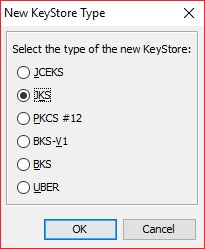
\includegraphics[width=0.5\textwidth]{../Dependancies/Keystore_Explorer/Type.jpg}
\end{figure}
  
\subsection{View and information}
You can view certificates and additional information with Keystore Explorer, view public and private key parts of certificates and other info such as subject alternative names by right clicking a certificate and choosing viable option from View option.

  \subsection{License}
Keystore Explorer is free to use utility, License is public.
  
\section{Generation and signing of certificates}

  \subsection{Keys, certificates and basic constraints}
  
    \subsubsection{Generate keys}
    
      \paragraph{Self-signed certificate}
It is possible to generate a key pair and self-signed certificate, simply click on icon or double click on blank space, choose algorithm and key length. Then you can choose all the other options such as Basic Constraints and Subject Alternative Name. \textit{(Figure 5.3)}

\begin{figure}[!ht]
 \caption{Generating keys}
 \centering
  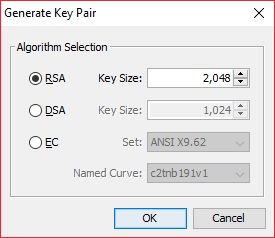
\includegraphics[width=0.5\textwidth]{../Dependancies/Keystore_Explorer/genKeys.jpg}
\end{figure}

\begin{figure}[!ht]
 \caption{Generating certificate}
 \centering
  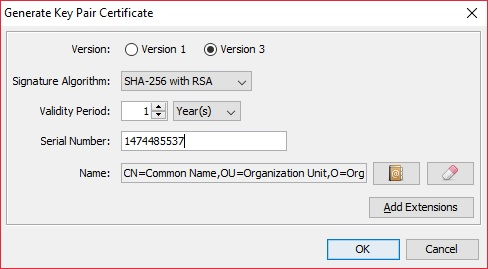
\includegraphics[width=0.5\textwidth]{../Dependancies/Keystore_Explorer/genCert.jpg}
\end{figure}

You can also set up default pre-fill of Common Name, Organisational Unit, Organisation etc.

      \paragraph{Certificate Signing Request}
It is possible to make Certificate Signing Request in Keystore Explorer. Simply generate key pair certificate and then right click the generated certificate and choose Generate CSR option. \textit{(Figure 5.4)}

\begin{figure}[!ht]
 \caption{Generating a CSR}
 \centering
  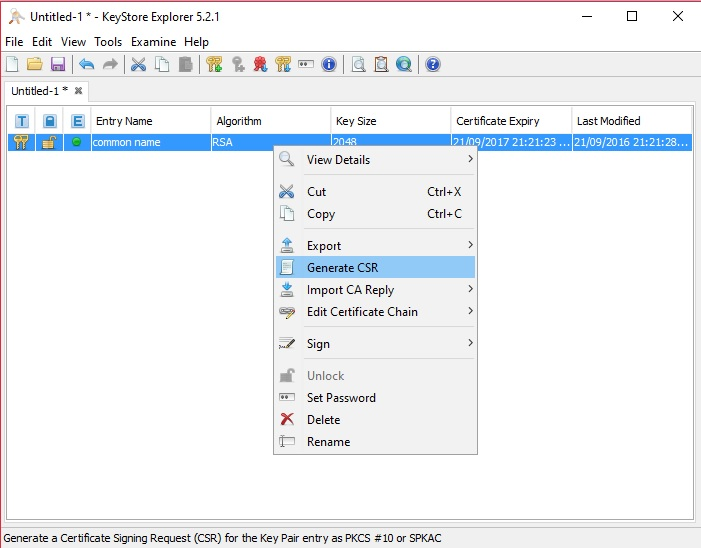
\includegraphics[width=0.5\textwidth]{../Dependancies/Keystore_Explorer/genCSR.jpg}
\end{figure}

      \paragraph{Specify length}
Length is specified at the moment of key pair generation.

      \paragraph{Specify algorithm}
Algorithm of keys is specified when generating keys and the certificate hash function is chosen by certificate authority.

    \subsubsection{Basic constraints}

\begin{figure}[!ht]
 \caption{Basic Constraints}
 \centering
  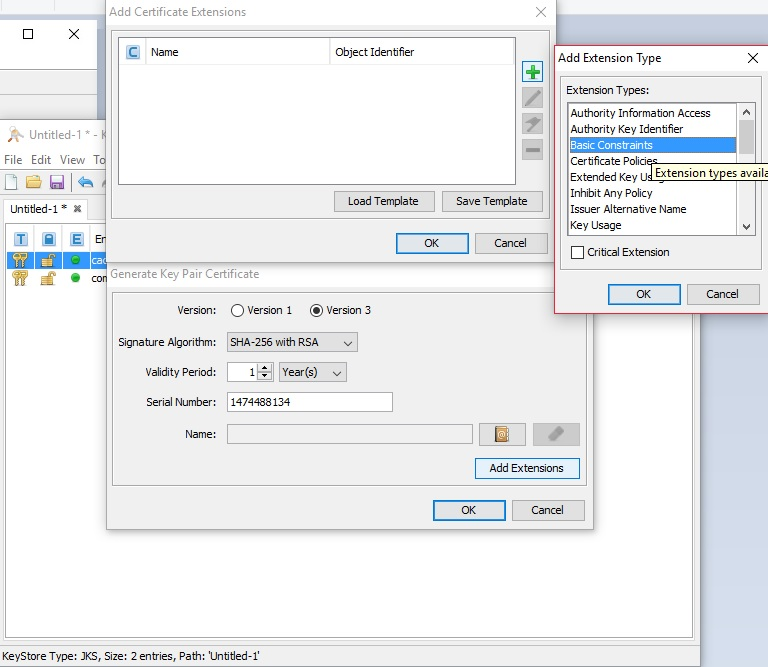
\includegraphics[width=0.5\textwidth]{../Dependancies/Keystore_Explorer/Basic_Constraints.jpg}
\end{figure}

      \paragraph{Specify Type}
Specifying type is made while generating keys and certificate by changing v3 portion when asked during generation.

      \paragraph{Specify path length}
Specifying of max path length is made also by changing v3 part of x509 certificate during generation under Basic Constraints type.\textit{(Figure 5.5)}

  \subsection{Specifications}
  
    \subsubsection{Certificate Signing Request signing}
To sign a Certificate Signing Request simply right-click a Certificate Authority certificate and use the \verb+sign->CSR+ option. Then you need to import CA response that was generated and saved in a desired place into a certificate from which the CSR was generated. \textit{(Figure 5.6)}

\begin{figure}[!ht]
 \caption{Signing of a CSR}
 \centering
  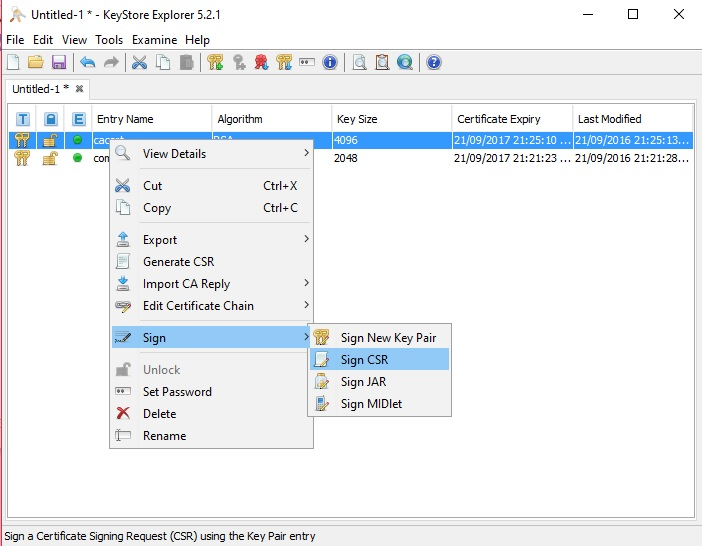
\includegraphics[width=0.5\textwidth]{../Dependancies/Keystore_Explorer/CSRsign.jpg}
\end{figure}

    \subsubsection{Create combination of private key and signed chain}
To create combination of private key and signed chain simply generate new key pair certificate, export private key part, import it back and then import to new certificate of private key a trusted chain.

    \subsubsection{Specify certificate validity}
Desired duration of certificate validity is asked during generation, but given whilst signing a Certificate Signing Request by Certificate Authority

    \subsubsection{Setting Subject Alternative Name for end certificates}
Setting of Subject Alternative Name for certificate is made during generation of certificate, under the add extentions option under the Subject Alternative Name part. Keystore Explorer allows to add both DNS and IP formats of SAN.

\section{Conversions}

  \subsection{Exporting}
  
    \subsubsection{Certificate or certificate chain from a file}
It is possible to export a certificate or certificate chain from a keystore by simply right-clicking the chosen certificate and chosing export option.

    \subsubsection{Private key only}
It is possible to export a private key from a keystore by simply right-clicking the chosen certificate and chosing \verb+export->private key+ option.

  \subsection{Direct conversion between Java Keystore and PKCS\#12 file}
To change a type of file simply right-click on the blank space and choose change type option. In addition to changing a pkcs12 file type to JKS it is possible to change type of files between all supported types of Keystore Explorer.
  
  \subsection{Importing certificates and keys into storage files}
It is possible to import certificates and keys by chosing Import option.

\chapter{XCA}

\section{General}

\textit{Tested under Windows 10 version 1607 Build 14393.447 and Fedora 21, XCA version 1.3.2 using OpenSSL version 1.0.2d}

  \subsection{Type}
XCA works with PKCS\#12 type files, but it is neccessary to make their database file which stores and to which you can import certificates, certificate signing requests or keys.
  \subsection{View and information}
You can view information about keys, certificates and CSRs by double clicking a chosen file.
  \subsection{License}
XCA is distributed under BSD License - it is free to use for testing and also commercially.
  
\section{Generation and signing of certificates}

  \subsection{Keys, certificates and basic constraints}
  
    \subsubsection{Generate keys}
    
      \paragraph{Self-signed certificate}
You can generate key pair by itself and then use it for generation of certificate. If you do not generate key in advance there is option to generate new key whilst generating a certificate.\textit{{Figure 6.1}}  \\


To generate a certificate click on Certificates tab and press New Certificate. There are many options for generating a self-signed certificate, under Source tab you choose a signing algorithm.  \\


Hash algorithm is one of: \verb+MD5, SHA1, SHA224, SHA256, SHA384, SHA512, RIPEMD160+. It needs to be changed because hash function is set to SHA-1 which is no longer considered safe.  \\


Under Subject tab, you shoose Common Name, Organisation, etc. fields of certificate and also choose private key. If you didn't generate key in advance then you can generate a new private key (\verb+RSA|DSA|EC+). For certificate to be accepted by all operating systems you need to choose \verb+Digital Signature & Key Agreement & Certificate Sign+ under Key usage tab. \textit{(Figure 6.2)}


\begin{figure}[!ht]
 \caption{Generation of key for new cert}
 \centering
  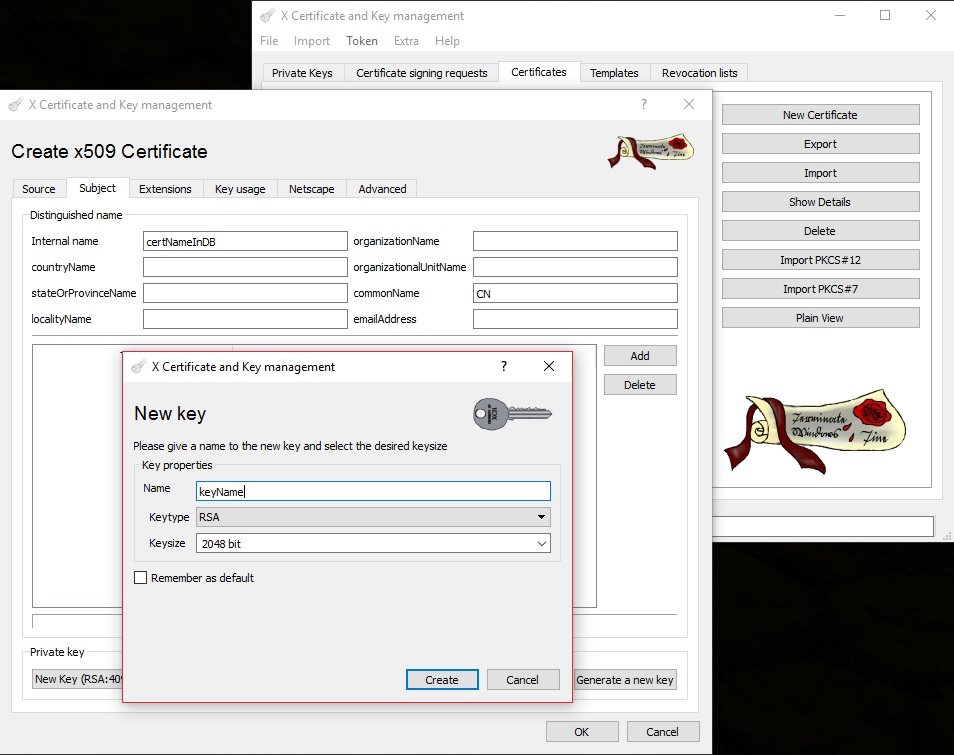
\includegraphics[width=0.5\textwidth]{../Dependancies/XCA/genKey.jpg}
\end{figure}

\begin{figure}[!ht]
 \caption{Specify usage}
 \centering
  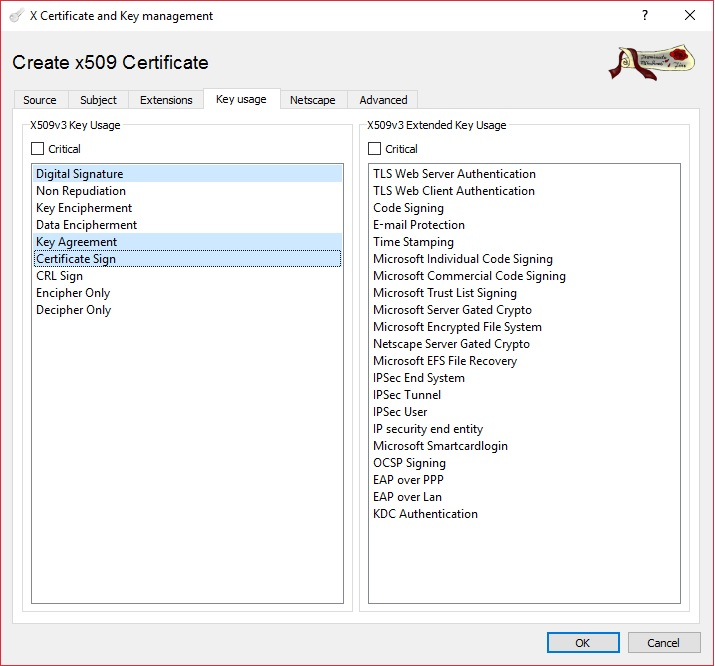
\includegraphics[width=0.5\textwidth]{../Dependancies/XCA/genKey_specif.jpg}
\end{figure}


      \paragraph{Certificate Signing Request}
Certificate Signing Request is generated similarly as a certificate itself, only difference is that you go under Certificate signing request tab and press New Request.
\begin{figure}[!ht]
 \caption{Generation of CSR}
 \centering
  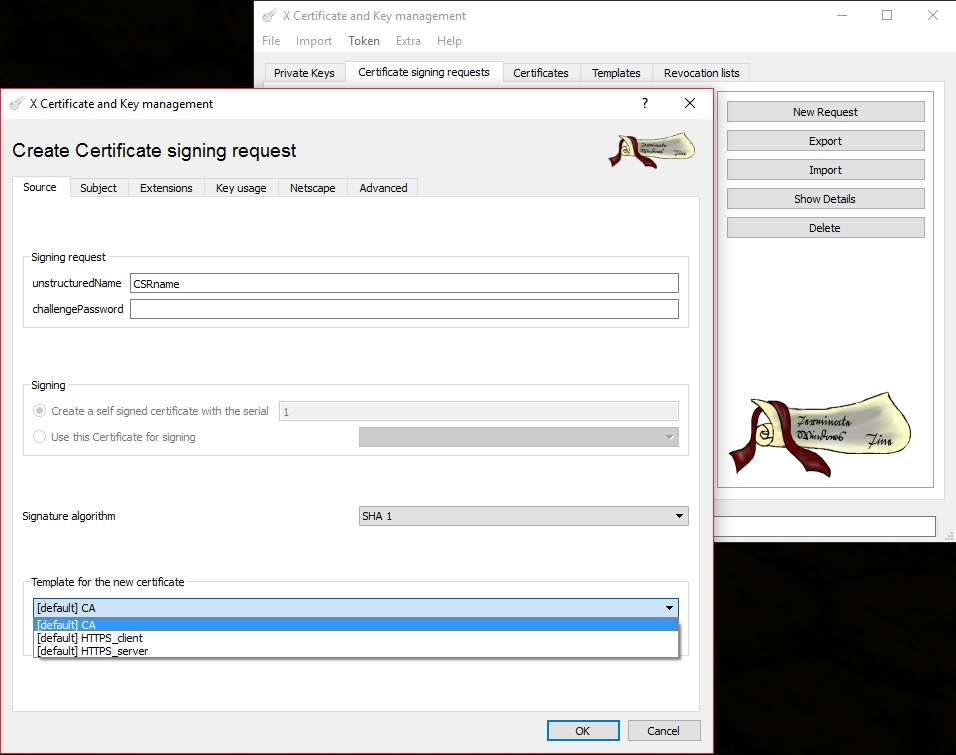
\includegraphics[width=0.5\textwidth]{../Dependancies/XCA/newCSR.jpg}
\end{figure}

      \paragraph{Specify length}
Length of keys is specified during generation of keys.
      \paragraph{Specify algorithm}
Algorithm used for key generation is specified during generation of keys (\verb+RSA|DSA|EC+).
\begin{figure}[!ht]
 \caption{Specifying of length and algorithm used}
 \centering
  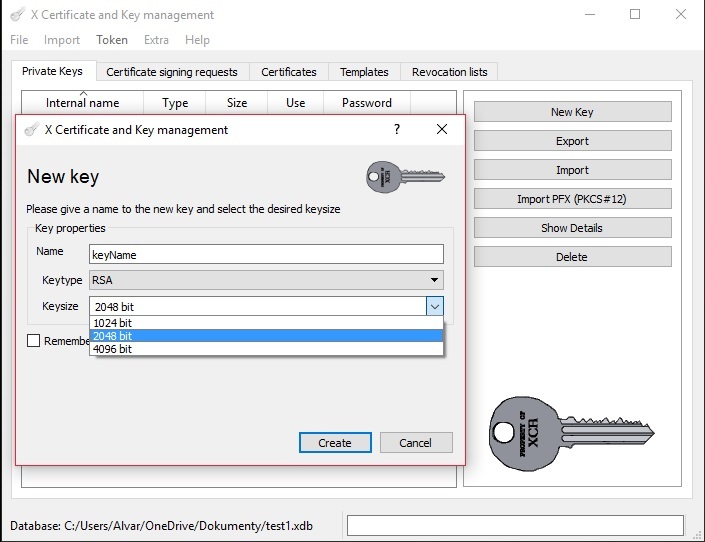
\includegraphics[width=0.5\textwidth]{../Dependancies/XCA/genKeylength.jpg}
\end{figure}


    \subsubsection{Basic constraints}
    
      \paragraph{Specify Type}
Type of a certificate is chosen under Extensions tab.
      \paragraph{Specify path length}
Path Length is also specified under Extensions tab.

\begin{figure}[!ht]
 \caption{Basic constraints, validity and SAN}
 \centering
  \includegraphics[width=0.5\textwidth]{../Dependancies/XCA/BC_ext.png}
\end{figure}

  \subsection{Specifications}
  
    \subsubsection{Certificate Signing Request signing}
To sign CSR you must have a CA certificate already in XCA's database. If a CA is availiable then you can sign CSR by:

\begin{enumerate}
\item using New Certificate option under Certificates tab 
\item right click on CSR under Certificate signing requests tab and choose Sign option. 
\end{enumerate}
Both options are equivalent.    

    \subsubsection{Create combination of private key and signed chain}
If the private key is provided PEM encoded it can be imported to XCA's database. If not you need to generate new key pair, then use export option to export private part of a key, delete key pair from database and then import private key. to create a combination, simply generate new certificate while using said private key.
    \subsubsection{Specify certificate validity}
Time period during which a certificate is valid is defined under Extensions tab.
    \subsubsection{Setting Subject Alternative Name for end certificates}
Subject Alternative Names are specified in appropriate section under an Extensions tab.
\textit{(Figure 6.5)}

\section{Conversions}

  \subsection{Exporting}
  
    \subsubsection{Certificate or certificate chain from a file}
Possible by using export option, choosing in which format you want to export it.

    \subsubsection{Private key only}
Exporting of private key only directly is availiable.

  \subsection{Importing certificates and keys into storage files}
Certificates and keys can be Exported and imported to/from PKCS\#12 or PEM type files.

\chapter{GnuTLS}

\section{General}

\textit{Tested under Fedora 21, certtool version 3.3.16}

  \subsection{Type}
GnuTLS works with PKCS\#12 PEM encoded files
  \subsection{View and information}
To view information about certificate use \verb+certtool --certificate-info --infile [file.pem]+ option.
  \subsection{License}
GnuTLS is under Gnu Public License \- free to use commercially.
  
\section{Generation and signing of certificates}

  \subsection{Keys, certificates and basic constraints}
  
    \subsubsection{Generate keys}
    
      \paragraph{Self-signed certificate}
To generate a self-signed certificate it is needed to generate a private key first. This is done by following command:
\begin{verbatim}
 certtool --generate-privkey --outfile [file.pem] --[rsa|dsa|ecc] \
          --sec-param=[low|legacy|medium|high|ultra]
\end{verbatim}
Where \verb+sec-param=<length_alias>+ and will be discussed in next parts.

To create a self-signed certificate with created private key use:
\begin{verbatim}
certtool --generate-self-signed --load-privkey ca-key.pem \
         [--template cert.cfg] --hash=[look@algorithm_part] --outfile ca-cert.pem
\end{verbatim}

More options when generating self-signed certificate (or a CSR) you need to create a config file which has structure as is in appendix \textit{GnuTLS.cfg} 
For whole list of options in a config file look up \verb+man certtool+.
      
\paragraph{Certificate Signing Request}
Creating of CSR is made by:
\begin{verbatim}
certtool --generate-request --load-privkey [keyfile.pem] \
         [--template cert.cfg]--outfile [csrfilename.pem]
\end{verbatim}

when not using template it asks for:
\begin{itemize}
\item Common Name, Organizational Unit, Organization, ...
\item Subject's domain component
\item Subject Alternative Name
\item If the certificate will be CA
\item What the certificate will be used for \textit{(signing $\vert$ encryption)}
\item Whether the certificate will be TLS web client/server certificate
\end{itemize}

\pagebreak

      \paragraph{Specify length}

Length is specified when generating keys by \verb+--sec-param=[low|legacy|medium|high|ultra]+ where length is determined by alias and algorithm.

\begin{table}[]
\centering
\caption{Bit length of security parameter options}
\label{my-label}
\begin{tabular}{|c|c|c|c|c|c|}
\hline
               & \textbf{low}      & \textbf{legacy}   & \textbf{medium}   & \textbf{high}     & \textbf{ultra}     \\ \hline
\textbf{RSA}   & \textit{1024 bit} & \textit{1776 bit} & \textit{2048 bit} & \textit{3072 bit} & \textit{15424 bit} \\ \hline
\textbf{DSA}   & \textit{1024 bit} & \textit{2048 bit} & \textit{2048 bit} & \textit{3072 bit} & \textit{3072 bit}  \\ \hline
\textbf{ECDSA} & \textit{160 bit}  & \textit{192 bit}  & \textit{224 bit}  & \textit{256 bit}  & \textit{512 bit}   \\ \hline
\end{tabular}
\end{table}

Also, to choose exact bit length you can use \verb+--bits=<length>+ option - tested on \verb+--rsa --bits=32768+ option which generated 32kbit RSA key.

      \paragraph{Specify algorithm}
Algorithm for key generation is specified in \verb+--[rsa|dsa|ecc]+ option where rsa = RSA, dsa = DSA, ecc = ECDSA.

To define a hash algorithm use \verb+--hash=[SHA1|RMD160|SHA256|SHA384|SHA512]+ option while generating a certificate.
    
  \subsubsection{Basic constraints}
    
      \paragraph{Specify Type}
To specify whether certificate should be CA or End cert write \verb+ca+ into the cert.cfg file and use that as a template for generation. 
      \paragraph{Specify path length}
Path length is specified by \verb+path_len=<value>+ option in cert.cfg file, where value is max chain length ( use -1 for undefined value).

  \subsection{Specifications}
  
    \subsubsection{Certificate Signing Request signing}
Possible by command:
\begin{verbatim}
certtool --generate-certificate --load-request <csr_file> \
         --load-ca-certificate <path_to_ca_cert> \
         --load-ca-privkey <ca_cert_privkey_file> 
         --outfile <name>.pem
\end{verbatim}

    \subsubsection{Specify certificate validity}
Validity is specified by changing cert.cfg file used while generating a certificate, the part \verb+expiration_days = <value>+
Alternatively, you cen set \verb+NOT BEFORE+ and \verb+NOT AFTER+ times by changing \verb+activation_date = <NOT_BEFORE_STRING>+ and \verb+expiration_date = <NOT_AFTER_STRING>+ where the times are written in GNU date string format.

    \subsubsection{Setting Subject Alternative Name for end certificates}
SAN is set by adding options to cert.cfg
\begin{verbatim}
dns_name = "www.dnsname1.com"
dns_name = "www.dnsname2.com"
  ...
dns_name = "www.lastdns.com"

uri = "uri1"
...

ip_address = "0.0.0.1"
ip_address = "0.0.0.2"
   ...
\end{verbatim}    

\section{Conversions}

  \subsection{Exporting}
  
    \subsubsection{Private key only}
It is not possible to export private key only, however for proper use of GnuTLS keys need to be stored on drive or imported to PKCS\#12 file.
  \subsection{Importing certificates and keys into storage files}
To import certificate and key into a PKCS\#12 file use command:
\begin{verbatim}
certtool --load-certificate <in_cert> \
         --load-privkey <in_key> \
         --to-p12 --outder --outfile <name>.[p12|pfx]
\end{verbatim}   



\chapter{Makecert and pvk2pfx}

\section{General}

\textit{Tested under MS Windows 10 version 14393.447, makecert.exe version 6.3.9600.17298} \\
Makecert is deprecated by Microsoft itself as cited on MSDN MakeCert site.

  \subsection{Type}
Makecert can work with PKCS\#12 type files, however  default output is in \verb+.cer+ for certificate and \verb+.pvk+ for private key. To tie together key and certificate you need to combine them into PKCS\#12 type file with \verb+pvk2pfx+ tool (which is also part of Windows SDK). In addition to use the tool you need to start a Developer Command Prompt for Visual Studio (on Windows 10). 

  \subsection{License}
It is free to use, falls under the Windows SDK.
  
\section{Generation and signing of certificates}

  \subsection{Keys, certificates and basic constraints}
  
    \subsubsection{Generate keys}

      \paragraph{Self-signed certificate}
Generating key and self-signed certificate that can be used as CA is not straightforward with Makecert.
\begin{verbatim}
makecert -n "CN=Common Name, OU=Organization Unit, O=..." -cy [authority|end] \
	 -a [sha256|sha384|sha512] -sv <key_file_name>.pvk -r \
	 -len <int key_length> <cert_name>.cer
\end{verbatim}

Where:
\begin{itemize}
\item \verb+-n+ sets credentials
\item \verb+-cy+ defines certificate type
\item \verb+-a+ chooses signature algorithm
\item \verb+-sv+ chooses name for file where the private key is stored
\item \verb+-r+ to create a self-signed certificate
\item \verb+-len+ for key length and without option choose the filename.
\end{itemize}

After entering this command you will be prompted to enter private key file password.

After creating certificate and private key file successfully to use self-signed certificate as a CA you need to join certificate file and private key into PKCS\#12 type file. This is made by using a pvk2pfx tool already implemented in Windows SDK.
\begin{verbatim}
pvk2pfx -spc <cert_file> -pvk <key_file>.pvk -pfx <pfx_file_name>.pfx \
        [-pi <key_password> -po <pfx_password]
\end{verbatim}

Where:
\begin{itemize}
\item \verb+-pi+ option is used if there is a password on key file
\item \verb+-po+ is desired pfx file password. If no password for pfx is given makecert defaults it to key file password.
\end{itemize}

      \paragraph{Specify length}
Length is specified by \verb+-len <int key_length>+ option.
      \paragraph{Specify algorithm}
To specify hash algorithm use \verb+-a [sha256|sha384|sha512]+ option. Supported are also SHA1 and MD5 but those are considered insecure.

To specify key algorithm you must change CSP.
    \subsubsection{Basic constraints}
    
      \paragraph{Specify Type}
It is possible with \verb+-cy [authority|end]+ option.

      \paragraph{Specify path length}
Path length is specified by \verb+-h <int length>+ option while creating a certificate.

  \subsection{Specifications}
  
    \subsubsection{Specify certificate validity}
Defaults from date of creation until 2039, to change use \verb+-b <mm/dd/yyyy -> from> -e <mm/dd/yyyy -> until>+ option.

Alternatively you can use \verb+-m <int months>+ option where you choose for how many months the certificate will be valid.

    \subsubsection{Support for Cryptographic Service Provider}
There is support for CSP in makecert by using \verb+-sp <provider_name> -sy <provider_type>+ defines the CryptoAPI provider for subject.
\section{Conversions}

  \subsection{Exporting}
  
    \subsubsection{Private key only}
Private key is stored and generated while generating a certificate but the type .pvk is uncommon.

  \subsection{Importing certificates and keys into storage files}
For importing of keys and certificates into PKCS\#12 file, use \verb+pvk2pfx+ as in generating self-signed part. There is just option to add 1 certificate and 1 private key into a file.


\chapter{Windows PowerShell PKI Module}

\textit{Tested under MS Windows 10 version 14393.447}

\section{General}

It should be noted that to be able to write into internal certificate storage, the PowerShell needs to be run as Administrator.
  \subsection{Type}
Windows PowerShell PKI Module works with Windows internal certificate storage but is able to export certificates in PKCS\#12 and DER formats. 
  \subsection{View and information}
To view information about certificates use \verb+Get-ChildItem -Path <path_to_cert>+ command where \verb+<path_to_cert>+ usually begins with \verb+Cert:\+ option.

This commands however show only thumbprint of certificate and a \verb+dns.name+. 
  \subsection{License}
License is Public, but working Microsoft Windows OS with PowerShell installed is needed.
  
\section{Generation and signing of certificates}

  \subsection{Keys, certificates and basic constraints}
  
    \subsubsection{Generate keys}
    
      \paragraph{Self-signed certificate}
To generate self-signed certificate use 
\begin{verbatim}
New-SelfSignedCertificate [-Provider <String>] -Path <storage_path> -DnsName "<cert_name>" 
\end{verbatim}

Where \verb+<cert_name>+ is used as Common Name for certificate. 

  \subsection{Specifications}
  
    \subsubsection{Setting Subject Alternative Name for end certificates}

If \verb+-DnsName <cert_name>+ is used as list of strings \textit{("dns1","dns2","dns3",...)} where \verb+dns2+ and latter are used as a Subject Alternative Name.    

    \subsubsection{Support for Cryptographic Service Provider}
Change of Cryptographic Service Provider is made by using \verb+-Provider <String>+ option.

\section{Conversions}

  \subsection{Exporting}
  
    \subsubsection{Certificate or certificate chain from a file}
Exporting of certificates is done by sequence:
\begin{verbatim}
$mypwd = Convert-To-SecureString -String "<password>" -Force -AsPlainText
Get-ChildItem -Path <path> | Export-PfxCertificate -FilePath <where_to_store> \
              [-ChainOption EndEntityCertOnly] [-Noproperties] -Password $mypwd
\end{verbatim}

Where:
\begin{itemize}
\item \verb+<password>+ will be password to created PKCS\#12 file as it is needed to export certificates and also needs to be of SecureString type.
\item \verb+<path>+ can be:
\begin{enumerate}
\item Path to certificate - only a specified certificate will be exported
\item Directory containing certificates \textit{e.g. Cert:{\textbackslash}LocalMachine{\textbackslash}My} - It will print all certificates into a single file
\end{enumerate}
\item \verb+<where_to_store>+ is location where the file will be saved.
\item \verb+[-ChainOption EndEntityCertOnly]+ if used only End certificates will be outputed and certificate chain will be ommited.
\item \verb+[-Noproperties]+ no additional properties will be printed out.
\end{itemize}

  \subsection{Importing certificates and keys into storage files}
It is possible in a simmilar way as exporting a certificate into PKCS\#12 file. Only difference is that all certificates that should be imported into a single folder and then \verb+<path>+ should be set to that directory. 
  
\part{Conclusion}

\chapter{Tools Review}

The main thing to understand is, that every tool has had its strong and weak points. Every should be used in complience with required properties of use.\\ 

That can mean restrictions on used Operating System \textit{(e.g. customer has only access to Apple computers with OS X operating system)}, or for example restrictions how it should be used on Operating System \textit{(command line vs GUI program)}. In the next part i will try to go over strengths and weaknesses of each tool that I have tested.

\section{OpenSSL}
It is a great command line tool, can work with PEM, DER and PKCS\#12 files. Strong point is an easy form of creating a self-signed certificate, however using it for CA certificates with ca option is not ideal -  creating CA is not advised in O'REILLY's Network Security with OpenSSL by J. Viega, M. Messier and P. Chandra on page 59,
\begin{displayquote}
\textit{Since OpenSSL's command-line CA functionality was intended primarely as an example of how to use OpenSSL to build a CA, we don't recommend that you attempt to use it in a large production environment.}
\end{displayquote}
and also hinted in manual pages:
\begin{displayquote}
\textit{The ca command is quirky and at times downright unfriendly.}

\textit{The ca utility was originally meant as an example of how to do things in a CA . It was not supposed to be used as a full blown CA itself: nevertheless some people are using it for this purpose.}

\textit{The ca command is effectively a single user command: no locking is done on the various files and attempts to run more than one ca command on the same database can have unpredictable results.}

\end{displayquote}


On the other hand strong point of OpenSSL is configuration of created certificate, which can be done in file. I tested it with creation of appropriate directories and configs.

\section{Keytool}
Keytool is the only command line tool using Java Keystore to store keys and certificates, which i consider it main strong point. By default the CSP is \verb+java.security.provider+ which allows RSA and DSA options and SHA-1,MD5,SHA-256 and SHA-512 hash algorithms. This changes when choosing other Cryptographic Service Provider. Working with it is quite easy and support for exporting as PKCS\#12 is usefull addition.

\section{GnuPG}
Tool that can only make end certificates for authentication, CSR is PEM encoded and does not hold generated private key inside. Unreliable as it has been tested on 5 different Operating Systems and worked only on clean install of Windows 8.1.

\section{Keystore Explorer}
A great GUI tool for when you need to work with different types of Java Keystore files. For example, Keystore Explorer supports Bouncy Castle implementation. Even though CSP support is not implicit, there are different choices already implemented. Those can be viewed under \verb+Help->Security Providers+ tab.

Main downfall is that keys of length greater than 4096 take longer to generate \textit{(notably RSA of length 16192, it took almost 2 hours to generate)}.

\section{XCA}
XCA is a great GUI tool that can work with PEM, DER and PKCS\#12 type of files. Main advantage is simplicity and amount of options, basic options are readily availiable as a button. There are many exporting options, for example PEM encoded certificate file with PKCS\#8 encrypted key file. Although there is no CSP support, its ease of use makes it a great testing tool.

\section{GnuTLS}
Command line tool, availiable only under Linux. Very friendly to use, many different options in configuration file. Great support for different key and hash algorithm types. Supports key lengths of higher values \textit{(greater than 4096 RSA for example)}. Its weaknesses are no support for CSP and availibility only under UNIX like Operating Systems.

\section{Makecert}
Command line tool, not to be used in production code since microsoft has deprecated it. Very unfriendly to use and only way to use it is to download a whole Windows SDK and use it with Visual Studio console. Overall it shouldn't be used.


\section{Windows PowerShell PKI Module}
PowerShell Module on Windows Operating Systems, much easier to use and generate new certificates. Downside is, that certificates made by it are RSAwithSHA256 2048bit and that can only be changed with change of Cryptographic Service Provider. It has replaced deprecated Makecert command line tool.

\chapter{Choosing the right tool}
The crucial part of deciding which tool to use is to know what is desired. The first choice to make is to decide what file type will be required.
In this list there are most useful tools for each type:

\begin{itemize}
 \item \textbf{PKCS\#12} \begin{enumerate}\item \textit{GUI} - XCA \item \textit{Command Line} - OpenSSL \end{enumerate}
 \item \textbf{Java KeyStore} \begin{enumerate}\item \textit{GUI} - Keystore Explorer \item \textit{Command Line} - keytool \end{enumerate}
\end{itemize}

Other tested tools can be also used, but \textit{OpenSSL, Keytool, XCA} and \textit{Keystore Explorer} can do almost everything, along with their ease of use. My personal favourite has become \textit{XCA} as it is a tool where I confirmed if information about certificates from other tools was as expected.\\

But only because they can do everything doesn't mean they are best at everything, for example if self-signed certificate is needed only for testing purposes, one can be really quickly made with the help of Windows PowerShell PKI Module where no additional instalations are required.\\

Considering Java KeyStore tools, only 2 were tested, 1 GUI and 1 Command Line. Nevertheless, even though they have their own upsides and downsides, are easy and quickly ready to use.\\

\end{document}
